\documentclass[conference]{IEEEtran}
\IEEEoverridecommandlockouts
% The preceding line is only needed to identify funding in the first footnote. If that is unneeded, please comment it out.
\usepackage{cite}
\usepackage{amsmath,amssymb,amsfonts}
\usepackage{algorithmic}
\usepackage{graphicx}
\usepackage{textcomp}
\usepackage{xcolor}
\def\BibTeX{{\rm B\kern-.05em{\sc i\kern-.025em b}\kern-.08em
    T\kern-.1667em\lower.7ex\hbox{E}\kern-.125emX}}
\begin{document}

\title{A Bayesian Approach to University Venue Allocation
}

\author{\IEEEauthorblockN{Mmasehume Raphiri}
\IEEEauthorblockA{\textit{School of Computer Science and Applied Mathematics} \\
\textit{The University of the Witwatersrand}\\
Johannesburg, South Africa \\
\email{mmasehume.raphiri1@students.wits.ac.za}}
\and
\IEEEauthorblockN{Ritesh Ajoodha}
\IEEEauthorblockA{\textit{School of Computer Science and Applied Mathematics} \\
\textit{The University of the Witwatersrand}\\
Johannesburg, South Africa \\
\email{ritesh.ajoodha@wits.ac.za}}}
\maketitle

\begin{abstract}
The University Venue Allocation Problem is a prominent and ever-increasingly NP-hard assignment problem in which students are assigned to available venues. A significant corpus of literature has explored various research directions to solve this problem. However, the uncertainty of conflicting constraints when solving the problem has not been probed extensively. This paper uses a Bayesian network (BN) modelling approach to address both uncertainty and causality in the venue allocation problem, and optimise the assignment of venues. Factors influencing venue allocation and the causal relationships between them were identified. Thereafter, a Bayesian Network structure of the problem is constructed. Data is then synthesized from the baseline model using BN forward propagation. Structure learning is carried out using a local search procedure (greedy hill-climbing) and Bayesian Parameter Estimation (BPE) is then used to learn the parameters of the model from the dataset. The model proposed in this paper is capable of resolving some of the most important issues with current venue allocation approaches by reducing uncertainty in expert evaluations and  modelling the causality between various sources of allocation uncertainty. Causal inference is performed to demonstrate the effectiveness of the model and the log-likelihood proves the validity of our approach.
\end{abstract}
\begin{IEEEkeywords}
Bayesian networks, University venue allocation, Uncertainty
\end{IEEEkeywords}

\section{Introduction}
The University Venue Allocation Problem, which is a subproblem of the University Course Timetabling Problem (UCTP), is a resource-constrained scheduling problem which involves the allocation of courses to venues, and possibly other resources subject to some constraints \cite{chen2020tabu}.

Effective course scheduling at universities is critical for optimal resource usage. Traditionally, the problem is tackled manually by trial and error, with no certainty of a valid and effective timetable solution \cite{basir2013simulated}. This may result in difficulties where the unavailability of a venue impacts the entire learning process, necessitating a manual rearrangement of the timetable. Even if a valid timetable solution is established, it is likely to raise the expense of the rescheduling procedure, and more crucially, it is likely to lose out on more effective options. As a result, these uncertainties have remained the primary motivation for scientific research on the problem.

The need for optimal teaching conditions in universities is another reason it is necessary to solve this problem. Too many students in small venues result in a decrease in the quality of learning, and students who require more support are often disregarded. Classes being allocated to venues that are too far away from each other leads to a needless waste of time since students and staff must walk to these remote venues.

Due to the prominence of the UCTP, numerous attempts have been made to either solve or provide more optimal solutions to the problem. These include a metaheuristic approach based on Simulated Annealing proposed by \cite{ceschia2012design} in post-enrollment course timetabling, a graph colouring approach by \cite{soni} and the genetic algorithm by \cite{lol}, \cite{ahmad}. 
% The proposed approach was evaluated on a benchmark dataset, which demonstrated that it was properly developed and modified. The proposed solution performed well on all datasets and produced new optimal solutions for the majority of the instances.

University venue allocation inevitably involves uncertainty. One or more of the following causes this uncertainty: 
\begin{itemize}
\item Causal relationships between constraints.
\item The number of available and required venues.
\item Occurrence of conflicting constraints.
\item The number of students to be enrolled.
\end{itemize}
Expert evaluations are often used to resolve uncertainty, but they are extremely subjective, which makes quantifying uncertainty challenging. Despite the variety of approaches to solving the venue allocation problem, this uncertainty has not been extensively studied in the current literature.

The most well-established approach to overcoming uncertainty in these circumstances is the Bayesian method \cite{efron2005bayesians}. The Bayesian approach is extended to situations involving intricate causal relationships through the use of Bayesian networks. Therefore, this paper proposes a Bayesian network approach to address the uncertainty and solve the venue allocation problem.

The main advantages of BNs that make them suitable for the university venue allocation domain are the following:
\begin{enumerate}
    \item BNs can make predictions with incomplete data. The total number of students that will be enrolled is usually unknown when venue assignments have to be made, this will encourage accurate assignments to still be created.
    \item BNs quantify uncertainty explicitly and simulate the causal relationship between variables. 
    \item BNs combine data from previous projects as well as expert opinions. Domain expertise could be utilized to determine whether critical data is lacking and whether the collected data is appropriate.
\end{enumerate}

The aim of this paper is to generate feasible venue assignments by learning the factors that influence uncertainty. To do so, we first define all the factors that influence venue allocation and use Bayesian structure learning to construct an allocation model, and thereafter, synthesise large amounts of data to train the model and get the conditional probability tables. Causal inference is conducted to check the robustness of the proposed approach and the log-likelihood score is calculated to prove the validity of our approach.

This paper provides the following contributions: (a) this paper provides a Bayesian network approach to solve the venue allocation problem; (b) a way to model the uncertainty and causality of the university venue allocation problem; (c) we provide a foundation for the development of new venue allocation solutions that are better informed and hence, are more useful and reliable.  

The rest of this paper is structured as follows: Section II reviews some of the current work in university timetabling and Bayesian scheduling; Section II highlights our research methodology, which includes a description of the data and testing of the model; and then, Section III and Section IV review the results and conclusion of this work respectively.

\section{Related Work}

Timetabling problems have been solved using a variety of algorithms. The earliest algorithmic approaches to the timetabling problem were derived from graph colouring heuristics. As seen in the work done by \cite{welsh1967upper}, these algorithms perform admirably in small instances of timetabling problems, but not in large ones. \cite{yu2002genetic} noted that the drawback of using graph colouring algorithms to solve timetabling problems is that they require the inclusion of non-academic limitations in problem formulation, which makes the solution hard to implement.

Recently, metaheuristic approaches have been extensively used to solve this problem and optimize timetable generation. Ant Colony Optimisation \cite{socha2002max}, \cite{cauvery2011timetable}, \cite{ceschia2012design}, \cite{nothegger2012solving} and Genetic Algorithms \cite{abdullah2007hybrid}, \cite{khonggamnerd2009improvement}, are some of the most well-known metaheuristics that have gotten the greatest attention from researchers and have been effectively applied to a wide range of optimization issues.

Timetabling problems have been reported to be solved by various combinations of population- and local-area-based algorithms in the literature \cite{tuga}, \cite{hao}, \cite{irene}. Due to the fact that population-based algorithms are more focused on exploration than exploitation, the quality of a solution generated by a population-based algorithm may not be superior to that of local-area-based algorithms.

\cite{bhagirathiautomatic} proposed a notable solution to the university venue allocation problem which utilizes a Bayesian Network. They represented the constraints of the problem as a Bayesian Network and learned the parameters of the network using Bayesian estimation. Their approach produced promising results but did not model the uncertainty of the problem. Therefore, this paper employs a Bayesian approach to quantify the uncertainty of the allocation problem, which is a useful addition and improvement to the metaheuristic and Bayesian methods previously studied. 

\section{Methodology}

To achieve the purpose of this research, the following research question will be explored:

Can a Bayesian network-based approach be used to solve the venue allocation problem?

To answer this question, firstly we will define all the factors that influence venue allocation and use Bayesian structure learning to construct an allocation model. Secondly, we synthesise large amounts of data to train the model and get the conditional probability tables. Lastly, we will evaluate the score of the learned model and do some casual inference to check the model's robustness.

To develop the proposed Bayesian network for university venue allocation, the following assumptions are made; students have already been assigned to courses, students and lecturers have no class preferences and time is a flexible constraint. These assumptions narrow down the scope of the problem and allow us to model it as just a venue allocation problem. 

The first one helps constrain the boundaries of our study domain to just university course timetabling compared to subject allocation. Then, the second assumption prevents us from modelling our problem as just a constraint satisfaction problem. Finally, the last one allows us to remove the added complexity that comes with assigning lectures into time slots.

A set of constraints must be satisfied by the final solution. The constraints are classified as either soft or hard constraints. The solution is feasible if it satisfies all the hard constraints.
Hard constraints are:
\begin{enumerate}
    \item Students can only attend one class at a time.
    \item A venue can accommodate only one class at a time.
    \item The number of seats in a venue should be sufficient for all students in a class.
\end{enumerate}

Soft constraints may be broken as long as the penalty cost is maintained low.
Soft constraints are:
\begin{enumerate}
    \item Venues should not be far away from each other.
    \item The number of empty seats should be minimized.
\end{enumerate}

\subsection{Data Collection and Pre-processing}
Since the university venue allocation problem, in general, is non-specific and different for each institution, the data used in this study is entirely synthetic. BN forward propagation was used to synthesise data. The baseline Bayesian network model was curated to model a situation that could occur in a university context so the data is not purely random.

The following steps are followed to generate the synthetic data:
\begin{enumerate}
  \item We designed a BN by creating a casual directed acyclic graph consisting of vertices and edges.
  \item A vertex is created for all the variables and the edges represent the independence assumptions between them. 
  \item Using the assumptions we inferred conditional probabilities between the variables.
  \item We simulate data using Bayesian network forward propagation.
\end{enumerate}

\begin{figure}[h]
    \center
  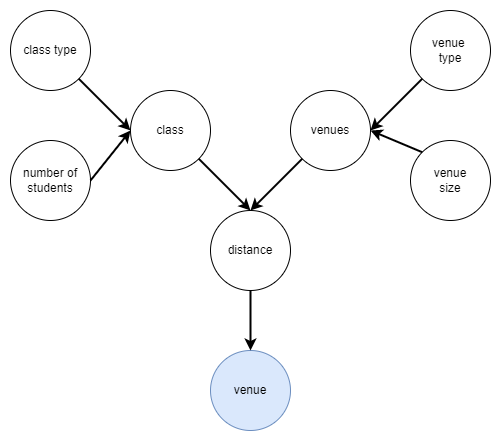
\includegraphics[scale=0.35]{images/Untitled Diagram.drawio (3).png}
  \caption{The Bayesian Network Structure for Venue Allocation}
  \label{fig:boat1}
\end{figure}

The data consists of a selection of classes to be assigned to appropriate venues. The classes are influenced by the number of students and the type of class they need to attend. The selection of venues is based on the size of the venue, the type of venue and the distance between venues. This is scalable because there is no limit to the number of classes that need to be assigned venues. The data is discrete and only has information about the occurrence of each variable. Since the data is synthetic, there was no need to do any explicit pre-processing.

\subsection{Model Representation}
The data used was sampled from a Bayesian network structure shown in Figure \ref{fig:boat1}. Each node represents a factor influencing venue allocation. The edges indicate that one node directly impacts the other node, while the absence of a directed edge indicates that the nodes are independent of one another. Bayes' Theorem, which is described in terms of conditional probability, is used to establish this causal relationship:

Where:
\begin{description}
    \item [$A$]: is the hypothesis.
    \item [$B$]: is the evidence.
    \item [$P(A)$]: is the likelihood of the hypothesis being true before the evidence is present.
    \item [$P(B)$]: is the likelihood of observing the evidence.
    \item [$P(B\vert A)$]: is the likelihood of observing the evidence if the  hypothesis is true.
\end{description}

The casual relationships are represented by conditional probability tables as seen in Figure \ref{fig:boat2}. 

\begin{figure}[h]
    \center
  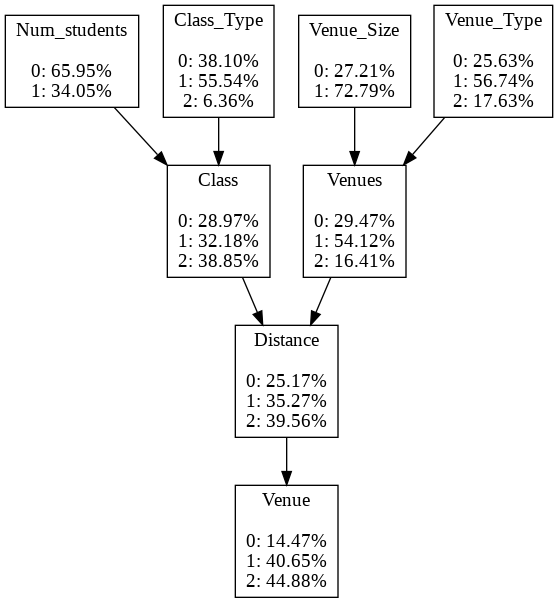
\includegraphics[scale=0.35]{images/download (1).png}
  \caption{Conditional Probability Tables}
  \label{fig:boat2}
\end{figure}

\subsection{Structure Learning}
The cornerstone of Bayesian network learning is structure learning, and effective structure learning is the key to building the optimal network structure since the network structure and data set can be used to determine the parameters.

Learning the structure of casual relationships between nodes is NP-hard. As a result, heuristic search methods are required.

Our search space consists of:
\begin{enumerate}
    \item a collection of DAGs that model the problem;
    \item a structure prior, which links our learned BNs together;
    \item a scoring function, we want to optimise;
    \item and finally, a search strategy which explores the search space.
\end{enumerate}


\textit{a) Search Procedure:} We used a greedy hill-climbing local search strategy. We randomly select an initial network and calculate the score of this network. We then iteratively try to improve the network by performing predetermined operators to get new networks. We compute the scores of the networks and the change that results in the best improvement to the score is implemented. Because the returned network structure may not always be the local optima, we used random restarts.

\textit{b) Scoring Function:} To measure the fit between the structure and the data, we used the Bayesian Information Criterion (BIC) score.
% the BIC score approximates ln p(D|Sh) as  , where  is an estimate of the model parameters for the structure, d is the number of model parameters, and N is the size of the dataset. 
%  The BIC score has a measure of how well the model fits the data, and a penalty term to penalise model complexity.


\subsection{Parameter Learning}
We train the BN classifiers to identify the ideal Bayesian structures by estimating a parameter set of joint probability distributions that best reflect supplied data set with labelled examples.

To learn the parameters of the model, we explored Maximum Likelihood Estimation (MLE) and Bayesian Parameter Estimation (BPE) and selected the best method to use based on the results from each approach. 

MLE estimates the parameters of the network, using the data set. To find the MLE we utilise the relative frequency, with which the variable states have occurred and fill the conditional probability tables (CPD) in such a way, that \textit{P(data$\vert$model)} is maximal. The problem with MLE is that it overfits data and when the observed data is not a representation of the underlying distribution, the MLEs are extremely inaccurate. As a result, MLE is extremely weak and unstable for learning network parameters.

To mitigate MLE's overfitting we compute the BPE. To find the BPE we start with previously existing CPDs that describe our ideas about the variables prior to data observation. The priors are then updated using state counts from the observed data. 

We make use of the Bayesian Dirichlet equivalent uniform (BDeu) prior which finds the Maximum a posteriori (MAP) structure, ensuring likelihood equivalence and equivalent sample size.

\subsection{Inference}
To demonstrate the effectiveness and evaluate the feasibility of our approach we do predictive inference. Bayesian prediction is based on the natural principle that newly collected evidence should be used to update predictions, and over time Bayesian predictions perform consistently well \cite{Sancetta}.

From the learned model, we estimate venue assignments by performing Variable Elimination (VE) and doing a maximum a posteriori probability (MAP) estimate query of the venue. 
Given an observation $B$, VE computes the posterior probability \textit{P(A$\vert$B = b)} from the Bayesian network structure. MAP maximizes this probability.

\subsection{Evaluation}
We evaluated how the model fits the data by performing a log-likelihood score. 
\section{Results}
All experiments were carried out on 10 same-sized data sets with 5 random restarts.
Table \ref{tab1} illustrates the averaged log-likelihood scores of the baseline model and the proposed model. Table \ref{tab1} suggests that using our proposed approach generates better models compared to the baseline.

We experiment with deleting random variables from the to see if our approach handles missing variables. Table \ref{tab2} shows the results of this experiment. Our approach still produces significant networks that are better than the baseline.

We used real-life university venue allocation examples to test whether or not the venue assignments predicted by the model satisfy all hard constraints. For all experiments, our approach produced feasible venue assignments.

These results show that our approach effectively models causality between different variables and uncertainty while producing a feasible solution.


\begin{table}[htbp]
\caption{Log likelihood Score Averaged Over 10 Runs}
\begin{center}
\begin{tabular}{|c|c|c|}
\hline
\textbf{Number of Samples} & \textbf{Baseline} & \textbf{BPE with BDeu} \\
\hline
% 0& 0 & 0 
% \hline
50& -396.7086 & -325.9922 \\
% \hline
100 & -576.8100 & -498.1301 \\
% \hline
200 & -886.0752 & -785.967 \\
% \hline
300 & -1213.8000 & -1106.6489\\
% \hline
400 & -1529.4773 &  -1414.5612\\
% \hline
500 &  -1881.4774 & -1756.5213\\
% \hline
600 & -2233.7893 & -2098.3670\\
% \hline
700 & -2571.5825 & -2437.0780\\
\hline
\end{tabular}
\label{tab1}
\end{center}
\end{table}

\begin{table}[htbp]
\caption{Log likelihood Score Averaged Over 10 Runs With Missing Variables}
\begin{center}
\begin{tabular}{|c|c|c|}
\hline
\textbf{Number of Samples} & \textbf{Baseline} & \textbf{BPE with BDeu} \\
\hline
% % 0& 0 & 0 \\
% \hline
50& -341.345 & -287.5893 \\
% \hline
100 & -524.8573 & -452.6630 \\
% \hline
200 & -773.8695 & -700.2863 \\
% \hline
300 & -1081.8857 & -986.5943\\
% \hline
400 & -1394.2310 &  -1284.3233\\
% \hline
500 &  -1688.0853 & -1571.4379\\
% \hline
600 & -1958.1887 & -1843.7448\\
% \hline
700 & -2269.3816 & -2145.7847\\
\hline
\end{tabular}
\label{tab2}
\end{center}
\end{table}

\section{Conclusion}
% This paper provided Bayesian network model-based approach to the  to quantify uncertainty.
The aim of this research was to solve the University Venue Allocation Problem using a Bayesian network model-based approach, with a strong focus on quantifying the uncertainty of the problem. This was achieved by modelling the problem as a Bayesian network with the factors influencing venue allocation represented as nodes. The structure and parameters of the network were then learned. This approach was able to successfully generate a feasible list of venue assignments and model the uncertainty of the problem.

To maximise the effectiveness of our technique, a more thorough investigation of parameter adjustment is required. Future work can take into student and lecture preferences to generate venue assignments that best suit them.

\begin{thebibliography}{00}
\bibitem{chen2020tabu} Chen, M., Tang, X., Song, T., Wu, C., Liu, S., \& Peng, X. (2020). A tabu search algorithm with controlled randomization for constructing feasible university course timetables. Computers \& Operations Research, 123, 105007.
\bibitem{lewis2008survey} A survey of metaheuristic-based techniques for university timetabling problems. OR spectrum, 30(1), 167–190.
\bibitem{basir2013simulated} Basir, N., Ismail, W., \& Norwawi, N. M. (2013). A simulated annealing for tahmidi course timetabling. Procedia Technology, 11, 437–445.
\bibitem{ceschia2012design} Ceschia, S., Di Gaspero, L., \& Schaerf, A. (2012). Design, engineering, and experimental analysis of a simulated annealing approach to the post-enrolment course timetabling problem. Computers \& Operations Research, 39(7), 1615–1624.
\bibitem{budiono2012pure} Budiono, T. A., \& Wong, K. W. (2012). A pure graph coloring constructive heuristic in timetabling. In 2012 international conference on computer \& information science (iccis) (Vol. 1, pp. 307–312).
\bibitem{efron2005bayesians} Efron, B. (2005). Bayesians, frequentists, and scientists. Journal of the American Statistical Association, 100 (469), 1–5.
\bibitem{welsh1967upper} Welsh, D. J., \& Powell, M. B. (1967). An upper bound for the chromatic number of a graph and its application to timetabling problems. The Computer Journal, 10 (1), 85–86.
\bibitem{yu2002genetic} Yu, E., \& Sung, K.-S. (2002). A genetic algorithm for a university weekly courses timetabling problem. International transactions in operational research, 9 (6), 703–717.
\bibitem{cauvery2011timetable} Cauvery, N. (2011). Timetable scheduling using graph coloring. International Journal of P2P Network Trends and Technology, 1(2), 57–62.
\bibitem{abdullah2007hybrid} Abdullah, S., Burke, E. K., \& McCollum, B. (2007). A hybrid evolutionary approach to the university course timetabling problem. In 2007 ieee congress on evolutionary computation (pp. 1764–1768).
\bibitem{khonggamnerd2009improvement} Khonggamnerd, P., \& Innet, S. (2009). On improvement of effectiveness in automatic university timetabling arrangement with applied genetic algorithm. In 2009 fourth international conference
on computer sciences and convergence information technology (pp. 1266–1270).
\bibitem{nothegger2012solving} Nothegger, C., Mayer, A., Chwatal, A., \& Raidl, G. R. (2012). Solving the post enrolment course timetabling problem by ant colony optimization. Annals of Operations Research, 194(1), 325–339.
\bibitem{socha2002max} Socha, K., Knowles, J., \& Sampels, M. (2002). A max-min ant system for the university course timetabling problem. In International workshop on ant algorithms (pp. 1–13).
\bibitem{bhagirathiautomatic} Bhagirathi, U. and Ajoodha, R. (2018). Automatic lecture, tutorial, and laboratory university venue allocation for varying
class sizes. Technical report, Honours Research Report, Faculty of Science, School of Computer Science and . . . 
\bibitem{Sancetta} A. Sancetta, “Universality of Bayesian Predictions”. Bayesian Analysis, Volume 7, pp. 1-36, 2012.

\bibitem{tuga}  M. Tuga, R. Berretta and A. Mendes, "A hybrid simulated annealing with kempe chain neighborhood for the university timetabling problem", Proc. 6th IEEE/ACIS Int. Conf. Comput. Inf. Sci., pp. 400-405, 2007.
\bibitem{hao} Z. L and J. K. Hao, "Adaptive tabu search for course timetabling", Eur. J. Oper. Res., vol. 200, no. 1, pp. 235-244, Jan. 2010.
\bibitem{irene} . S. F. H. Irene, S. Deris and S. Z. M. Hashim, "A study on PSO-based university course timetabling problem", Proc. Int. Conf. Adv. Comput. Control, pp. 648-651, 2009. 
\bibitem{ahmad} Ahmad I,S Sufahani , Ali M and Razili C (2017). A Heuristics Approach for Classroom Scheduling Using Genetic Algorithm Technique. IOP Conf. Series: Journal of Physics: Conf. Series 995 (2018) 012050.

\bibitem{soni} Soni, A., Ajoodha, R. and Padayachee, K., A Solution to the University Timetabling Problem using Graph Colouring.
\bibitem{lol} M. Fachrie and A. F. Waluyo, "Guided Genetic Algorithm to Solve University Course Timetabling with Dynamic Time Slot," 2020 3rd International Seminar on Research of Information Technology and Intelligent Systems (ISRITI), 2020, pp. 583-587, doi: 10.1109/ISRITI51436.2020.9315448.
\end{thebibliography}
\end{document}
